\lecture{6}{jeudi 26 mars 2020}
\vspace{-1.2cm}

\section{The Marketing Funnel}

Le marketing (ou purchase) funnel est un outil qui permets de visualiser, d'un point de vue théorique, la customer journey de l'achat d'un produit ou service. Le premier modèle, développé en 1898 par Elias St. Elmo Lewis est le modèle AIDA.
\vspace{-0.7cm}

\begin{minipage}[t]{0.4\textwidth}
\begin{figure}[H]
\hspace{-2cm}
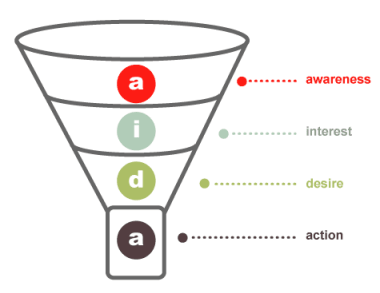
\includegraphics[scale=0.60]{../images/lec6img1}
\end{figure}
\end{minipage}
\begin{minipage}[t]{0.7\textwidth}
\vspace{1.8cm}
\begin{itemize}
\item \textbf{Awareness:} Le prospect va être amené à se rendre compte d'un potentiel problème qu'il a et des solutions qui existent;
\item \textbf{Interest:} Le prospect va exprimer son intérêt pour un groupe de produits ou services qui peuvent résoudre son problème;
\item \textbf{Desire:} Le prospect va exprimer son intérêt pour un produit ou service spécifique et va commencer à évaluer si celui-ci correspond à ses besoins;
\item \textbf{Action:} Le prospect décide de si oui ou non le produit ou service correspond à ses besoins et devient soit un client (si oui), ou va continuer ses recherches (si non).
\end{itemize}
\end{minipage}
\vspace{0.2cm}

Depuis, ce modèle a beaucoup évolué, mais les principes de base restent les mêmes. Aujourd'hui, quand on parle de funnel marketing, on va essentiellement parler d'un modèle où il y a 3 catégories. Chacune de ces catégories apporte son approche de communication différentes:

\begin{itemize}
    \item \textbf{TOFu - Top Of the Funnel - Awareness Stage:} construire la notoriété sur le produit/service et le problème qu'il est sensé adresser de façon assez large.
    \item \textbf{MOFu - Middle Of the Funnel - Consideration Stage:} apporter un peu plus d'informations sur l'utilité du produit/service et comment il est utilisé.
    \item \textbf{BOFu - Bottom Of the Funnel - Decision Stage:} expliquer en quoi votre solution est la meilleure. \\
\end{itemize}

Analysons chacune de ces phases plus en détail\\

\textbf{The awareness stage}

\begin{itemize}
    \item Objectif: Se positionner comme étant une solution valable et avantageuse. Pour le faire, il faut d'abord amener les potentiels clients sur le site web et espérer réussir à les faire souscrire à une newsletter ou toute autre forme de source de contact régulier.
    \item Contenu à produire: Campagnes de pub, blog posts, contenu sur le site web, webinars, guides d'utilisation, posts sur les réseaux sociaux, newsletters.
    \item KPIs à observer: Traffic sur le site web (visites et visites uniques), "social reach", nombre de personnes qui souscrivent à la newsletter, liens entrants, référencement.\\
\end{itemize}

\textbf{The consideration stage}

\begin{itemize}
    \item Objectif: Nourrir les leads avec du contenu qui prouve que l'entreprise est capable de résoudre leur problème.
    \item Contenu à produire: Études, outils gratuits, livres blancs, webinars.
    \item KPIs à observer: Pourcentage d'ouverture des emails, conversion rate sur la landing page, lead source, coût par lead.\\
\end{itemize}

\textbf{The decision stage}

\begin{itemize}
    \item Objectif: Persuader les leads à cliquer sur le bouton "buy", ou du moins rentrer en contact avec les équipes sales ou les magasins.
    \item Contenu à produire: Témoignages d'utilisateurs, études comparatives de produits, démonstrations, temps d'évaluation gratuite, offre personnalisée.
    \item KPIs à observer: Conversion rate du lead-to-sale, revenu, coûts engrangés pour obtenir le client.\\
\end{itemize}

Une autre évolution postérieure à celle-ci a été proposée, rajoutant deux étapes en plus: la Loyalty (rester en contact avec ses consommateurs même après leur achat pour rester dans leur esprit et potentiellement trigger des nouveaux achats ultérieurs) et l'Advocacy (créer une relation assez forte avec ses consommateurs pour qu'ils recommandent le produit/service à d'eux mêmes à d'autres personnes). La raison de l'ajout de ces deux étapes est simple: des recherches indiquent qu'une simple augmentation de 5\% pour la customer retention peut augmenter les profits d'une entreprise de 95\%. \\

\subsection{Customer Conversion Funnel}

\begin{figure}[H]
\hspace{-2cm}
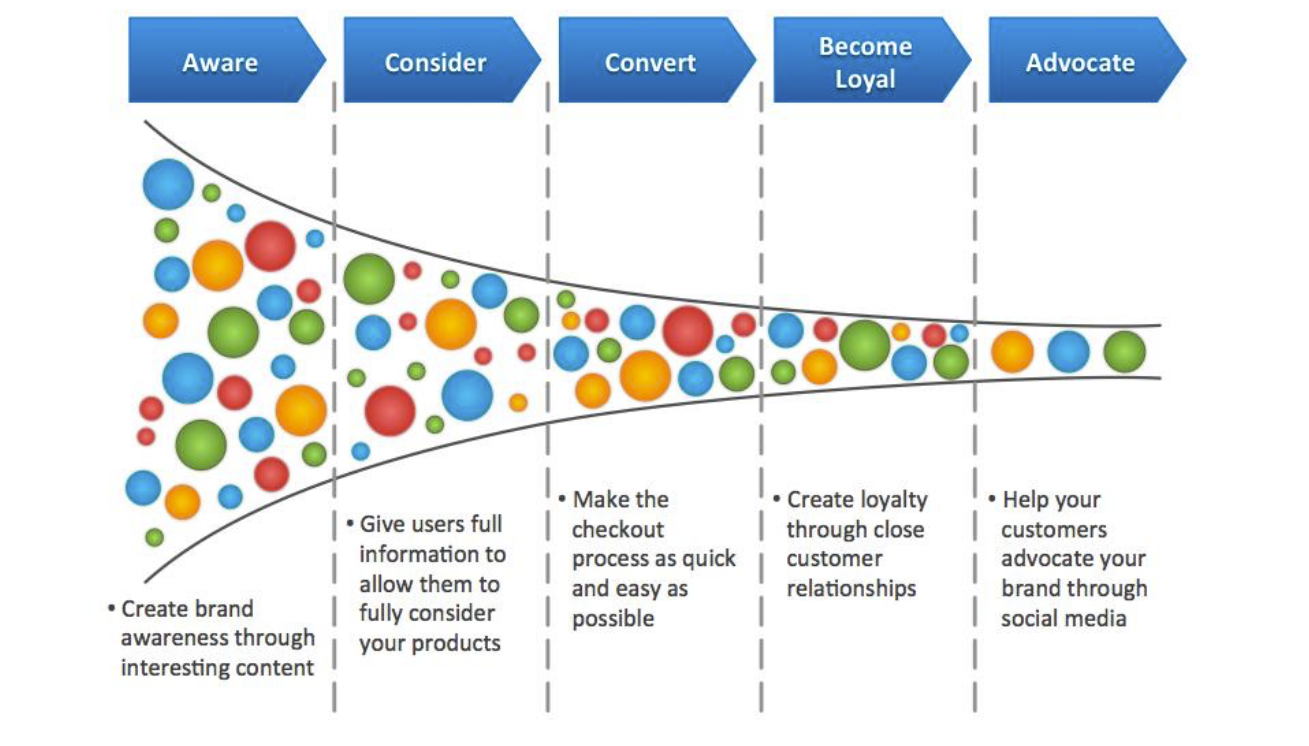
\includegraphics[scale=0.40]{../images/lec6img2}
\end{figure}

Le Customer Conversion Funnel est une phrase utilisée dans le e-commerce pour décrire la customer journey d'un client depuis une publicité sur internet ou lien cliqué sur un moteur de recherche, puis navigation sur le site de e-commerce, et conversion finale en vente.\\

La conversion d'un visiteur sur internet à une vente est un effort considérable, à toutes les étapes. Lors d'un exemple vu au cours, on peut passer de 100.000 fans Facebook à seulement 5 ventes. La perte de personnes à chaque étape peut être due à plein de raisons: peu de gens voient effectivement le post facebook, peu de gens cliquent sur le lien, peu de gens trouvent ce qu'ils veulent et l'ajoutent dans leur "cart", certains ne passent même pas au checkout, et dans ceux-là certains ne payent finalement pas. Il faut donc vraiment trouver plein de façons d'augmenter la conversion rate à chaque étape.\\

\newpage
\subsection{MQL VS SQL}

Il faut bien faire la différence entre un MQL (Marketing Qualified Lead) et un SQL (Sales Qualified Lead). \\

Le MQL est une personne qui peut potentiellement devenir un client. Pour s'assurer qu'une personne est un MQL il faut vérifier que le produit/service que l'entreprise propose est un bon match avec cette personne. Il faut assigner un certain nombre de points aux actions possibles qu'une personne peut avoir vis à vis du contenu proposé par l'entreprise (ouverture d'email, chat sur les réseaux sociaux, téléchargement de contenus informatifs sur le site, remplissage d'un) et, si l'on remarque que la personne dépasse un certain seuil de nombre de points, ils peuvent être considérés comme des MQL.\\

Le SQL est une personne qui a montré un grand intérêt pour le produit/service et également un intérêt à acheter. Ils ont peut-être même besoin de faire cet achat dans un futur proche. Tandis qu'il est possible de définir un MQL de façon automatisée avec un software, pour un SQL c'est légèrement plus compliqué. Typiquement c'est quelque chose qui est issu d'une discussion entre un lead et une personne de l'équipe sales. La chose la plus important est que lorsqu'on a détecté qu'une personne est un SQL, il faut absolument qu'un sales prenne les devants et essaye de répondre à toutes les questions qu'elle aurait, pour peu à peu la convaincre d'acheter.\\

\subsection{Conversion rates et personnalisation}

\textbf{Stratégie CRO}

La Conversion Rate Optimisation (CRO) est le procédé d'optimisation d'un site web pour agrandir le nombre de visiteurs qui deviennent des leads ou clients par la suite.\\

\textbf{CTR}

Le Click-Through-Rate est le rapport entre le nombre de clics sur le nombre d'impressions et se calcule comme ceci : CTR = (Nombre de clics / Nombre d'impressions ) x 100.

Les différents médias ont des CTR très différents. Par exemple, une pub internet banale a un CTR de 0,05\%, une bannière de 0,13\%, les ad words de 3,17\% et une publicité dans les réseaux sociaux entre 0,5\% et 1,6\%. Ces chiffres sont vraiment petits quand on les compare à des médias plus anciens tels que les newsletters (5\%) ou le courrier papier (6,2\%).
